\documentclass[22pt]{article} 
\usepackage{geometry} 
\usepackage{float} 
\usepackage{graphicx}
\usepackage{caption}
\usepackage{subfigure}
\usepackage{amsmath}
\usepackage{array}
\geometry{left=2.0cm,right=2.0cm,top=0.5cm,bottom=2cm}
	\author{Mengfan Wang} 
	\title{Stochastic Signal Systems Homework 2} 
\begin{document}
		\maketitle 
	\paragraph{1}
		\subparagraph{a} $S_Y = \{0\leq Y \leq 1\}$.
		\subparagraph{b} The equivalent event is: A point is selected uniformly at random from inside the circle with the radius $y$.
		\subparagraph{c} \begin{align} 
				 P[Y\leq y] = 
				\begin{cases}
				1 & y>1\\
				y^2 & 0\leq y \leq 1 \\
				0 & y<0
				\end{cases}
		\end{align}

	\paragraph{2}
		\begin{align}
		P(A) & = 1 - P[\{X\leq 1/3\}] = 1 - F_X(1/3) = 0\\
		P(B) & = 1 - P[\{|X|<1\}] = 1 - [F_X(1^{-})-F_X(-1)] = 1 - (1 - 1/3) = 1/3\\
		P(C) & = F_X(4/3^-) - F_X(-2/3) = 16/27\\
		P(D) & = F_X(0^-) = 1
		\end{align}

	\paragraph{3}
		\subparagraph{a}
		\begin{align}
			\int_0^{10} k + 0.25 \delta(x-5) + 0.25 \delta(x-10) dx &= 1\\
			10k + 0.5 & = 1\\ 
			k & = 0.05
		\end{align}
		\subparagraph{b} 
						\begin{align}
						P[X\leq	5] = \int_0^{5} 0.05 + 0.25 \delta(x-5) + 0.25 \delta(x-10) dx  = 0.5\\
						P[5\leq X <10]=\int_5^{10} k + 0.25 \delta(x-5) + 0.25 \delta(x-10) dx -f_X(10)&= 0.5\\
						\end{align}
		\subparagraph{c}\begin{figure}[H]
				\centering
				\subfigure{
					\begin{minipage}{9cm}
					\centering 
					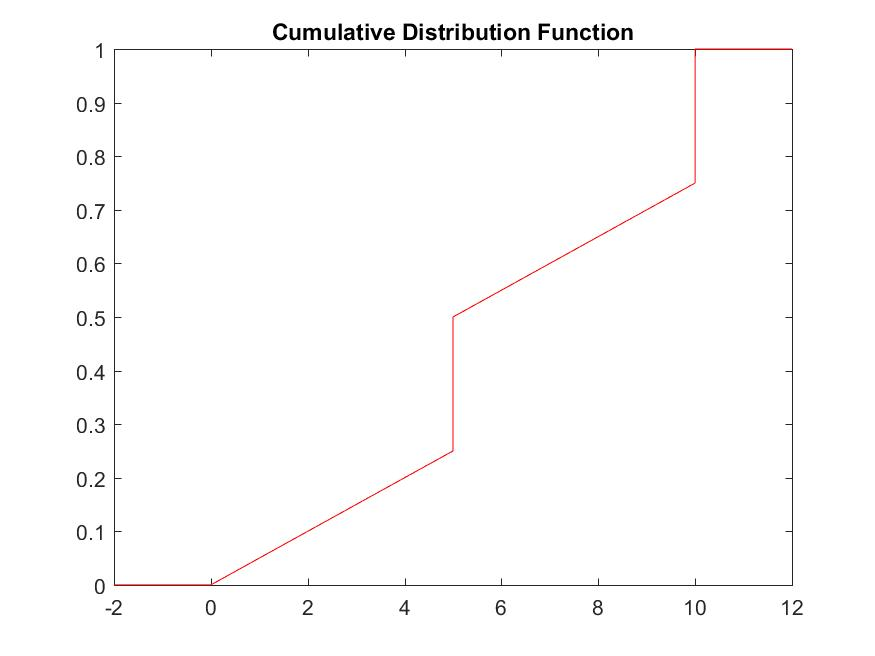
\includegraphics[height=6cm]{3.jpg}
					\end{minipage}
				}
				\caption{The cumulative distribution function of $f_X(x)$} 
			\end{figure}


		\paragraph{4} Firstly, because $U$ is uniformly distributed between zero and one, we have $P[U\leq x] = x$ when $0\leq x \leq 1$.
		Then we have:
		\begin{align}
		F_Y(y) & = P[Y\leq y]\\
		& = P[F_X^{-1}(U)\leq y]\\
		& = P[U\leq F_X(y)]\\
		& = F_X(y) \label{4}
		\end{align}
		Eq.\ref{4} is correct because $0\leq F_X(y) \leq 1$. So, $Y$ has the same distribution as $X$.

		\paragraph{5}Suppose $t\geq	0$ for all questions.
			\subparagraph{a}  When $x \leq t$, $F_X(x|X>t) =0$; When $x \geq t$, we have:
			\begin{align}
				F_X(x|X>t) &= \frac{P[\{X\leq x\}\cap\{X >t\}]}{F_X(X>t)}\\
				& = \frac{F_X(t<X\leq x)}{F_X(X>t)} \\
				& = \frac{1-e^{-\lambda x}-1+e^{-\lambda t}}{e^{-\lambda t}}\\
				& = 1 - e^{-\lambda(x-t)}
			\end{align}
			So, \begin{align} 
				 F_X(x|X>t) = 
				\begin{cases}
				0 & x< t\\
				1 - e^{-\lambda(x-t)} & x\geq t
				\end{cases}
		\end{align}
		Figure \ref{5a} shows the corresponding plot. $F_X(x|X>t)$ equals to $F_X(x)$ which translated to right with the distance $t$. That is, $F_X(x|X>t) = F_X(x-t)$.
		\begin{figure}[H]
				\centering
				\subfigure{
					\begin{minipage}{9cm}
					\centering 
					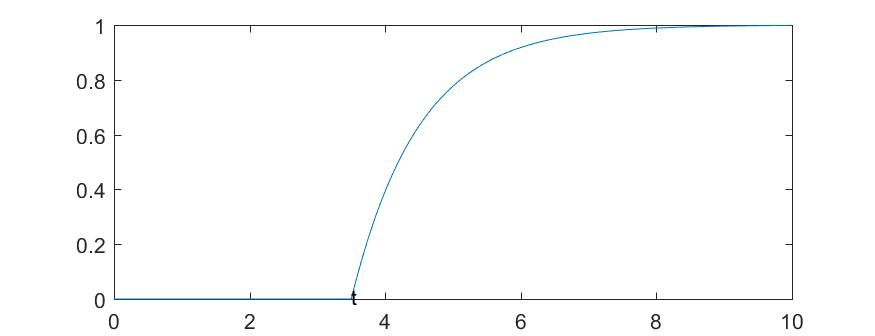
\includegraphics[height=4cm]{5a.jpg}
					\end{minipage}
				}
				\caption{The figure of $F_X(x|X>t)$. Set $t = 3.5$ and $\lambda = 0.5$. } 
				\label{5a}
			\end{figure}

			\subparagraph{b} $f_X(x|X>t) = \frac{d}{dx}F_X(x|X>t) = \lambda e^{-\lambda(x-t)}$ when $x \geq t$.
			So,
			\begin{align}
				f_X(x|X>t) = 
				\begin{cases}
				0 & x< t\\
				\lambda e^{-\lambda(x-t)} & x\geq t
				\end{cases}
			\end{align}
			\begin{figure}[H]
				\centering
				\subfigure{
					\begin{minipage}{9cm}
					\centering 
					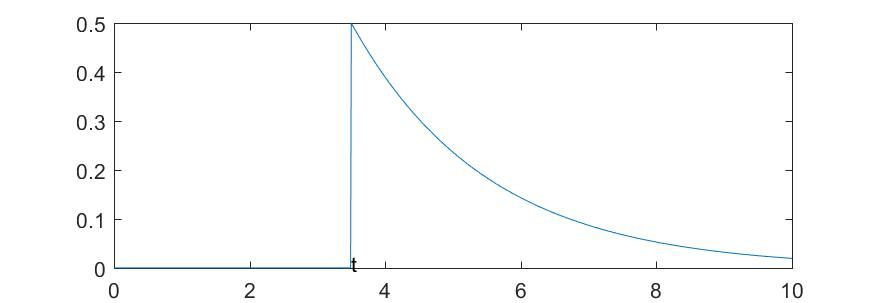
\includegraphics[height=4cm]{5b.jpg}
					\end{minipage}
				}
				\caption{The figure of $f_X(x|X>t)$. Set $t = 3.5$ and $\lambda = 0.5$. } 
				\label{5b}
			\end{figure}
		\subparagraph{c}
		\begin{align}
		P[X>x]  & = 1 - F_X(x) = 1 - (1 - e^{-\lambda x}) = e^{-\lambda x} \\
		P[X>t+x|X>t] & = \frac{P[\{X>t+x\}\cap \{X>t\}]}{P[X>t]} = \frac{1-F_X(t+x)}{1-F_X(t)} = \frac{e^{-\lambda(t+x)}}{e^{-\lambda t}} = e^{-\lambda x}
		\end{align}
		So we have $P[X>t+x|X>t]=P[X>x]$. It means no matter how to change $t$, the probability that the random variable $X$ is larger than $x$ is unchanged. If $t$ represents the time, it means the future status of this system is independent to its history. That's why it's termed memoryless property.

		\paragraph{6}
				\subparagraph{a}
				When $-\pi/2<x<\pi/2$, we have $F_X(x) = \int_{-\frac{\pi}{2}}^{x} \frac{1}{2}cos(x) = \frac{1}{2}sin(x) + \frac{1}{2}$. So,
				\begin{align}
				F_X(x) = 
				\begin{cases}
				0 & x\leq \pi	/2\\
				\frac{1}{2}sin(x) + \frac{1}{2} & -\pi	/2<x<\pi	/2\\
				1 & x\geq \pi	/2
				\end{cases}
			\end{align}

			\subparagraph{b}
			\begin{align}
			P(A) & = F_X(\pi/6) - F_X(0^-) \\
			& = \frac{1}{2}sin(\pi/6) -\frac{1}{2}sin(0)\\
			& = 1/4
			\end{align}
			\subparagraph{c} When $X \in A$: 
			\begin{align}
			F_X(x|A) & = \frac{P[\{X\leq x\}\cap\{A\}]}{P[A]}\\
			& = \frac{P[{0\leq X \leq x}]}{1/4}\\
			& = 2sin(x)
			\end{align}
			So, the cdf of $X$ is:
			\begin{align}
				F_X(x|A) = 
				\begin{cases}
				0 & x<0\\
				2sin(x) & 0 \leq x \leq \pi	/6\\
				1 & x>\pi/6
				\end{cases}
			\end{align}

		\subparagraph{d} 
					\begin{align}
					f_X(x|A) = \frac{d}{dx} F_X(x|A)=
					\begin{cases}
					0 & x<0 \quad or \quad x>\pi	/6\\
					2cos(x) & 0 \leq x \leq \pi	/6\\
					\end{cases}
				\end{align}

		\paragraph{7}
		\begin{align}
		& P[A|X\leq x]F_X(x) + P[A|X\geq x](1-F_X(x)) \\
		= & \frac{P[A\cap\{X\leq x\}]}{P[X\leq x]}P[X\leq x] + \frac{P[A\cap\{X> x\}]}{P[X> x]}P[X>x]\\
		= & P[A\cap\{X\leq x\}] + P[A\cap\{X> x\}]\\
		= & P[A]
		\end{align}

		\paragraph{8} \begin{align}
			f_X(x|(X-10)^2<4) & = \frac{d}{dx}F_X(x|(X-10)^2<4) \\
			& = \frac{d}{dx}\frac{P[\{X\leq x\}\cap (X-10)^2<4]}{P[(X-10)^2<4]}
		\end{align}
		When $x\leq 8$, $P[\{X\leq x\}\cap (X-10)^2<4] = 0$; When $x\geq 12$, $P[\{X\leq x\}\cap (X-10)^2<4] = P[(X-10)^2<4]$; Otherwise, $P[\{X\leq x\}\cap (X-10)^2<4] = F_X(x)-F_X(8)= \Phi(x-10)-\Phi(-2)$, while $P[(X-10)^2<4]=\Phi(2)-\Phi(-2)$.
		So we have:
		\begin{align}
				f_X(x|(X-10)^2<4) & = \frac{d}{dx}\frac{P[\{X\leq x\}\cap (X-10)^2<4]}{P[(X-10)^2<4]} \\
				& = \begin{cases}
				0 & (x-10)^2 \geq 4\\
				\frac{1}{\sqrt{2 \pi}(\Phi(2)-\Phi(-2))}exp(-\frac{(x-10)^2}{2})  & (x-10)^2 <4
				\end{cases}
			\end{align}

		\paragraph{9}
		\subparagraph{a}
		\begin{align}
		\sum_{k=-\infty}^{\infty}P[N=k] & = \sum_{k=1}^{\infty}P[N=k] = 1\\
		\sum_{k=1}^{\infty} c/k^2 & = 1\\
		c \pi	^2/6 & = 1\\
		c = 6/\pi^2
		\end{align}

		\subparagraph{b} $P[N = 1] = 6/\pi^2$,$P[N = 2] = 3/(2\pi^2)$,$P[N = 3] = 2/(3\pi^2)$,$P[N = 4] = 3/(8\pi^2)$.
		So we have
		\begin{align}
				P[N = k|N \leq 4] = 
				\begin{cases}
				0 & k< 1 \quad or \quad k>4\\
				\frac{144}{205k^2} & 1\leq k \leq 4 
				\end{cases}
			\end{align}

		\paragraph{10}
			\subparagraph{a} 
				When $x>0$, $F_X(x|\{X>0\}) = \frac{P[\{X\leq x\}\cap \{X>0\}]}{P[X>0]} = 1 - e^{-2x}$. 
				So,
				\begin{align}
				F_X(x|\{X>0\}) = 
				\begin{cases}
				0 & x\leq 0\\
				1 - e^{-2x} & x>0
				\end{cases}
			\end{align}

			\subparagraph{b}
			\begin{align}
				F_X(x|\{X=0\}) = 
				\begin{cases}
				0 & x< 0\\
				1 & x\geq0
				\end{cases}
			\end{align}

		\paragraph{11}
			\subparagraph{a} According to the total probability theorem, we have:
			\begin{align}
			P[X\leq x] & = \sum_{k=1}^{n}P[X\leq x|A_k]P(A_k)\\
			F_X(x) & = \sum_{k=1}^{n}F_X(x|A_k)P(A_k)
			\end{align}
			And, 
			\begin{align}
			f_X(x) &= \frac{d}{dx}F_X(x)\\
			& = \sum_{k=1}^{n}f_X(x|A_k)P(A_k)
			\end{align}

			\subparagraph{b}
			\begin{align}
			P[A|x_1<X\leq x_2] & = \frac{P[x_1<X\leq x_2|A]P[A]}{P[x_1<X\leq x_2]}\\
			& = \frac{F_X(x_2|A)-F_X(x_1|A)}{F_X(x_2)-F_X(x_1)}P[A]
			\end{align}

			\subparagraph{c}From Eq. (2) we have:
			\begin{align}
			P[A|x<X\leq x+\Delta x] &=\frac{F_X(x+\Delta x|A)-F_X(x|A)}{F(x+\Delta x)-F(x)}P[A] \\
			\lim_{\Delta x \rightarrow 0} P[A|x<X\leq x+\Delta x]& =\lim_{\Delta x \rightarrow 0} \frac{F_X(x+\Delta x|A)-F_X(x|A)}{F(x+\Delta x)-F(x)}P[A] \\
			P[A|X=x] & = \lim_{\Delta x \rightarrow 0}  \frac{F_X(x+\Delta x|A)-F_X(x|A)}{\Delta x}\lim_{\Delta x \rightarrow 0}\frac{\Delta x}{F(x+\Delta x)-F(x)}P[A]\\
			P[A|X=x] & = \frac{d}{dx} F_X(x|A)\frac{1}{\frac{d}{dx}F_X(x)}P[A]\\
			P[A|X=x] & = \frac{f_X(x|A)}{f_X(x)}P[A]
			\end{align}
			So, 
			\begin{align}
			f_X(x|A) = \frac{P[A|X=x]}{P[A]}f_X(x)
			\end{align}
			Then we have:
			\begin{align}
			P[A]f_X(x|A) & = P[A|X=x]f_X(x)\\
			\int_{-\infty}^{\infty} P[A]f_X(x|A) dx& =\int_{-\infty}^{\infty} P[A|X=x]f_X(x)dx\\
			P[A]\int_{-\infty}^{\infty} f_X(x|A) dx& =\int_{-\infty}^{\infty} P[A|X=x]f_X(x)dx\\
			P[A]& =\int_{-\infty}^{\infty} P[A|X=x]f_X(x)dx
			\end{align}






\end{document}